\section{Testing di Usabilità}

\subsection{Metodologia di Valutazione dell'Implementazione}
La valutazione condotta in questo capitolo si configura come una \textbf{Valutazione dell'implementazione}, in quanto coinvolge gli utenti finali in interazioni dirette con il sistema software parzialmente funzionante (nel caso del portale Web) e con un prototipo ad alta fedeltà (nel caso dell'applicazione Mobile).

Seguendo il framework \textbf{DECIDE} \cite{preece2015interaction}, gli obiettivi principali ad alto livello della valutazione sono stati: misurare il livello di usabilità del prodotto, verificare il raggiungimento degli obiettivi pre-fissati e identificare eventuali criticità nell'interazione con i flussi principali.

Per rispondere a queste domande, è stato adottato un approccio ibrido che combina tecniche osservazionali e interrogative. È stato condotto un test simulato su un campione di 10 utenti: 5 focalizzati sulle funzionalità Web (dedicate a enti e curatori) e 5 sulle funzionalità Mobile (dedicate ai turisti).

\subsubsection{Tecniche adottate durante e dopo il test}
\begin{itemize}
    \item \textbf{Valutazione Cooperativa (Variazione del Think Aloud):} Durante l'esecuzione dei task, gli utenti sono stati incoraggiati a descrivere a voce alta le proprie azioni e a criticare costruttivamente l'interfaccia. Il valutatore è intervenuto solo nei momenti di impasse per indagare a fondo sulle difficoltà percepite.
    \item \textbf{Questionario di Usabilità (SUMI):} Al termine del test pratico, è stato impiegato il \textbf{SUMI (Software Usability Measurement Inventory)} \cite{kirakowski1993sumi}. Si tratta di un questionario standardizzato composto da 50 item (sia a valenza positiva che negativa) progettato per misurare oggettivamente la soddisfazione dell'utente e l'usabilità globale del software lungo cinque dimensioni: Efficienza, Affettività, Utilità, Controllo e Apprendibilità. Sono state inoltre incluse domande aperte per raccogliere feedback qualitativo.
\end{itemize}

\subsection{Risultati del Questionario e Analisi dei Dati}
I dati quantitativi raccolti attraverso il SUMI sono stati normalizzati su una scala da 0 a 100 per ottenere un indice di usabilità globale e per analizzare le specifiche dimensioni dell'interazione. I punteggi mostrano un livello di soddisfazione complessivamente molto elevato per entrambe le piattaforme, a dimostrazione di una progettazione solidamente incentrata sull'utente.

Come evidenziato dal primo grafico riportato in appendice a questo capitolo (Figura \ref{fig:sumi_global}), le due piattaforme si attestano su livelli di usabilità globale eccellenti e pressoché identici, confermando l'efficacia delle soluzioni adottate sia per l'applicativo Web che per quello Mobile. L'analisi di dettaglio sulle 5 Dimensioni del SUMI (Figura \ref{fig:sumi_dimensions}) permette di osservare variazioni più sottili: l'Efficienza e il Controllo si confermano robusti su entrambi i fronti, mentre l'Affettività (ovvero il coinvolgimento emotivo) registra punteggi molto alti per il Mobile, giustificati dall'uso di tecnologie immersive come la Realtà Aumentata e il Narratore. 

Il questionario ha rivelato inoltre (Figura \ref{fig:sumi_importance}) che la quasi totalità del campione ritiene il software valutato come "Importante" o "Estremamente Importante" per lo svolgimento delle proprie attività (turistiche o gestionali), sottolineando la reale utilità e l'alto livello di empowerment generato dal sistema Culturia.

\subsection{Analisi Critica dell'Esperienza Utente}
Dall'analisi incrociata tra i dati quantitativi e le preziose risposte aperte fornite dagli utenti a fine questionario, sono emersi chiari punti di forza e aree di miglioramento che guideranno i futuri cicli di sviluppo.

\textbf{Punti di forza emersi (Miglioramenti Apprezzati):}
\begin{itemize}
    \item \textbf{Lato Web (Enti e Curatori):} Gli utenti hanno elogiato in particolar modo la semplicità nel creare nuovi tour turistici e l'intuitività della pagina di personalizzazione dedicata al proprio ente museale. Anche la chiara separazione logica introdotta per il caricamento delle fonti storiche è stata valutata molto positivamente.
    \item \textbf{Lato Mobile (Turisti):} Il feedback più entusiasta ha riguardato il \textit{Narratore in Realtà Aumentata (AR)}, che rende l'esplorazione sul campo estremamente immersiva. Inoltre, l'inserimento dei meccanismi di gamification è stato riconosciuto come un forte incentivo per visitare un numero maggiore di opere.
\end{itemize}

\textbf{Punti da migliorare (Sviluppi Futuri Identificati):}
\begin{itemize}
    \item \textbf{Lato Web:} Nonostante l'apprezzamento generale, la composizione strutturale delle singole tappe di un tour risulta a tratti macchinosa e richiede un'ulteriore semplificazione. È emersa inoltre la forte necessità di integrare un portale di verifica o un sistema di consigli automatici per coadiuvare la ricerca e la validazione delle fonti documentali.
    \item \textbf{Lato Mobile:} Alcuni utenti hanno segnalato che l'albero di navigazione del menu principale è migliorabile in termini di intuitività. Ulteriori richieste si sono concentrate sulla semplificazione della funzione di ricerca per le opere d'arte e sulla necessità di una gestione più chiara degli eventi temporanei associati agli enti museali.
\end{itemize}

\subsection{Relazione sul Testing di Usabilità}
In conclusione, la campagna di testing ha confermato la validità architetturale e concettuale del sistema \textit{Culturia}, registrando un altissimo grado di soddisfazione tra gli utenti intervistati. I pochi ostacoli rilevati nell'interazione non precludono il raggiungimento degli obiettivi primari dei task, ma rappresentano preziosi spunti di ottimizzazione. 

Come sviluppo futuro, ci si prefigge di risolvere le criticità emerse (in particolare lo snellimento dei flussi lato Web e il miglioramento della navigazione lato Mobile) e di condurre una nuova e più estesa fase di sperimentazione. Quest'ultima vedrà il software testato nel pieno delle sue funzionalità definitive su una base di utenti significativamente più ampia, al fine di consolidare i risultati ottenuti.

\newpage
\subsection*{Grafici dei Risultati}
\vspace{-0.5cm}

\begin{figure}[H]
    \centering
    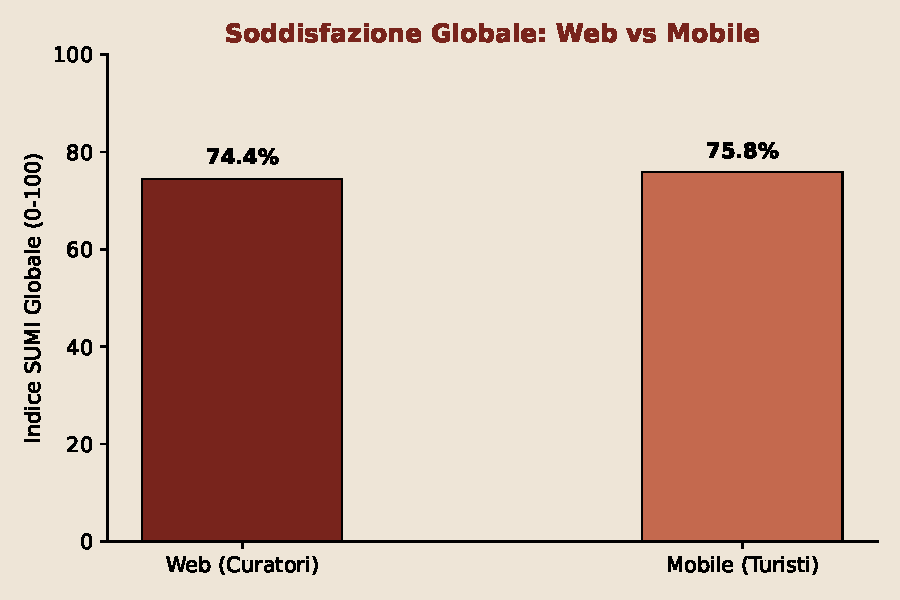
\includegraphics[width=0.55\textwidth]{figures/sumi_global.pdf}
    \caption{Indice SUMI Globale per le piattaforme Web e Mobile}
    \label{fig:sumi_global}
\end{figure}
\vspace{-0.4cm}

\begin{figure}[H]
    \centering
    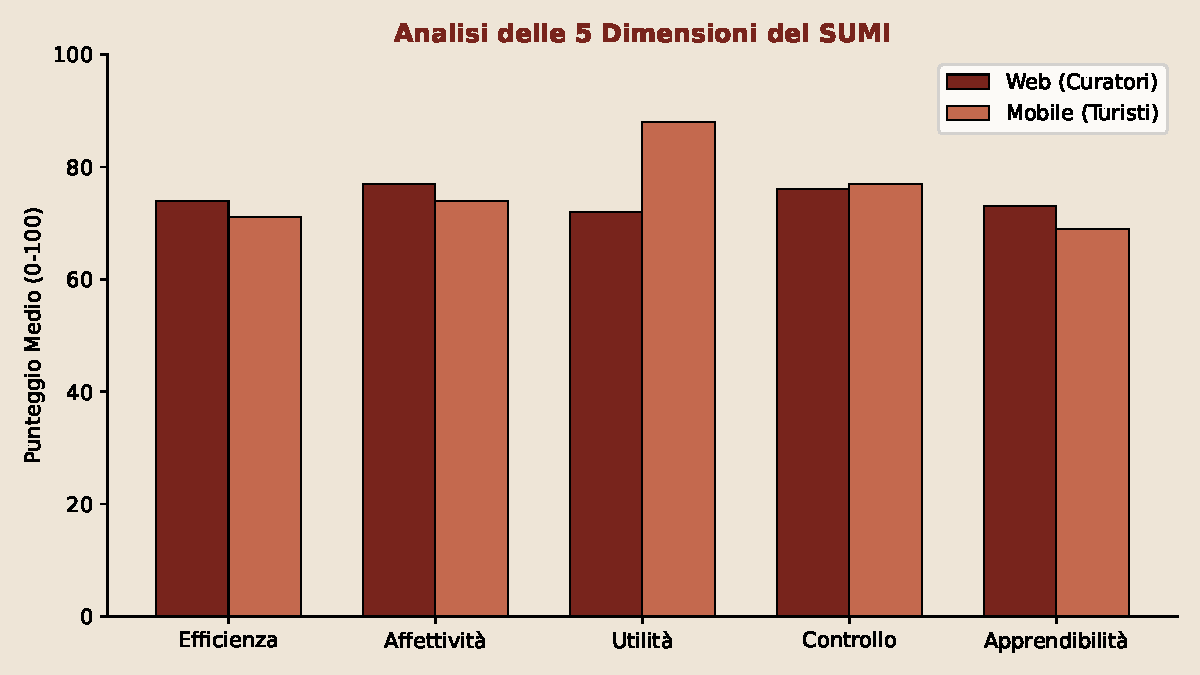
\includegraphics[width=0.65\textwidth]{figures/sumi_dimensions.pdf}
    \caption{Analisi delle 5 Dimensioni dell'Usabilità SUMI (Web vs Mobile)}
    \label{fig:sumi_dimensions}
\end{figure}
\vspace{-0.4cm}

\begin{figure}[H]
    \centering
    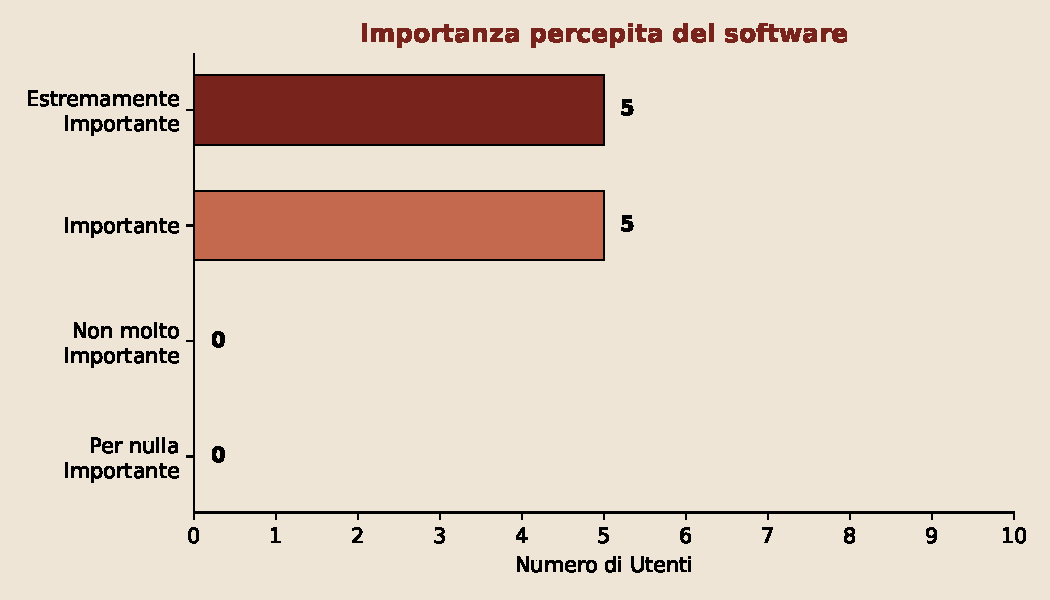
\includegraphics[width=0.6\textwidth]{figures/sumi_importance.pdf}
    \caption{Importanza del software}
    \label{fig:sumi_importance}
\end{figure}

\newpage
\section{Valutazione dell'Empowerment}

Al termine della fase di testing di usabilità e della compilazione del questionario SUMI, gli stessi 10 utenti reali coinvolti nella sperimentazione sono stati invitati a compilare un ulteriore questionario incentrato sull'Empowerment. 

Questo strumento di indagine è stato strutturato in modo del tutto analogo al questionario somministrato durante le fasi iniziali del progetto (Assignment 1), con una differenza fondamentale: in questa occasione, le domande sono state declinate per valutare in modo specifico l'esperienza diretta degli utenti con il sistema \textit{Culturia} ormai funzionante. 

L'obiettivo di questa fase finale di valutazione è stato quello di misurare l'effettivo livello di \textit{empowerment} raggiunto, confrontando le aspettative iniziali con i benefici reali percepiti nell'utilizzo della piattaforma, sia dal punto di vista gestionale (per i curatori) che da quello esperienziale (per i turisti).

